%\documentclass{article}

%\usepackage{graphicx}
%\usepackage{enumitem}

%\begin{document}

% Nama Kelompok : Kelompok 2
% Kelas : D4 TI 1A
% 1. Kadek Diva Krishna Murti (1174006)
% 2. Duvan Silalahi (1174011)
% 3. Oniwaldus (1174005)
% 4. Choirul Anam (1174004)
% 5. Sri Rahayu (1174015)
% 6. Ilham Habibi (1174028)

\section{Pengertian Sensor Suara}

\begin{figure}[ht]
\centerline{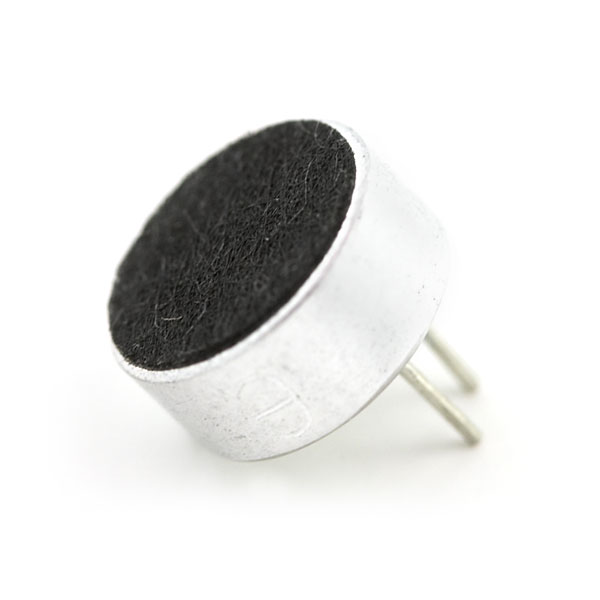
\includegraphics[width=0.4\textwidth]{figures/sscondesermic.jpg}}
\caption{Condeser Microphone}
\label{condesermic}
\end{figure}

Sensor suara merupakan sensor yang mensensing besaran suara untuk diubah menjadi besaran listrik. Sensor ini bekerja berdasarkan besar kecilnya kekuatan gelombang suara yang diterima. Dimana gelombang suara tersebut mengenai membran sensor, yang menyebabkan bergeraknya membran sensor yang memiliki kumparan kecil sehingga menghasilkan besaran listrik. Kecepatan bergeraknya kumparan kecil tersebut menentukan kuat lemahnya gelombang listrik yang akan dihasilkan. Salah satu contoh komponen yang termasuk dalam sensor ini adalah condeser microphone atau mic. Bentuk fisik dari condeser mic yaitu berbentuk bulat dan memiliki kaki dua seperti contoh pada gambar \ref{condesermic}.

\section{Prinsip Kerja Condeser Microphone}

\begin{figure}[ht]
\centerline{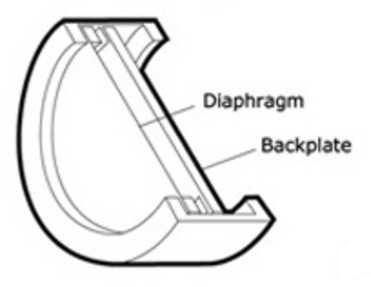
\includegraphics[width=0.4\textwidth]{figures/sscondesermicscheme.jpg}}
\caption{Skema dari Condeser Microphone}
\label{condesermicscheme}
\end{figure}

Condenser mic biasanya bekerja berdasarkan susunan backplate atau diafragma yang harus terhubung dengan listrik dan membentuk kapasitor sound - sensitive. Gelombang suara yang tercipta akan masuk ke microphone dan akan menggetarkan komponen diafragma ini. Letak dari diafragma ditempatkan di depan sebuah backplate. Susunan dari elemen - elemen tersebut akan membentuk sebuah kapasitor yang sering disebut juga sebagai kondenser. Kapasitor memiliki kemampuan untuk menyimpan muatan maupun tegangan. Ketika elemen tersebut terisi dengan muatan, medan listrik akan terbentuk di antara diafragma dan backplate, yang dimana besarnya itu proporsional terhadap ruang yang terbentuk diantaranya. Macam - macam lebar dari jarak antara backplate dengan diafragma yang terjadi disebabkan karena adanya pergerakan oleh diafragma relatif terhadap backplate yang dikarenakan adanya tekanan suara yang mengenai diafragma. Hal ini akan menghasilkan sinyal elektrik dari gelombang suara yang masuk ke condenser microphone seperti contoh pada gambar \ref{condesermicscheme}.

\section{Karakteristik dari Condeser Microphone}

\hspace{4mm} Karakteristik dari Conseder Microphone adalah sebagai berikut :

\begin{itemize}
\item Susunannya lebih kompleks dibanding dengan jenis microphone lainnya seperti dibanding dengan dynamic Microphone.
\item Pada frekuensi tinggi, akan menghasilkan suara yang lebih halus dan natural, serta sensitivitas yang lebih tinggi.
\item Mudah akan mencapai respon frekuensi flat dan memiliki range frekuensi yang lebih luas.
\item Ukurannya lebih kecil dibanding dengan jenis tipe mikrophone lainnya.
\end{itemize}

Pada pasaran sudah dijual sensor suara menggunakan condeser mic ini dalam bentuk modul, sehingga mudah dan praktis dalam penggunaannya.

\section{Spesifikasi dari Modul Sensor Suara}

\begin{figure}[ht]
\centerline{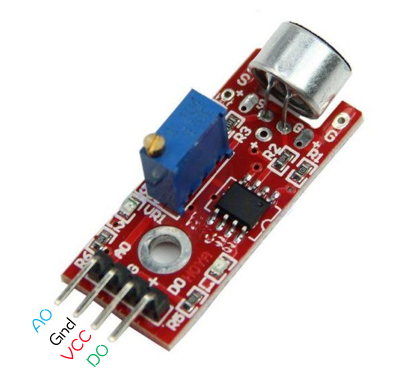
\includegraphics[width=0.4\textwidth]{figures/sssensorsuara.png}}
\caption{Modul Sensor Suara}
\label{sssensorsuara}
\end{figure}

Spesifikasi dari modul sensor suara seperti contoh pada gambar \ref{sssensorsuara} adalah sebagai berikut :

\begin{itemize}
\item Sensitivitas dapat diatur (pengaturan manual pada potensiometer).
\item Condeser yang digunakan memiliki sensitivitas yang tinggi.
\item Tegangan kerja antara 3.3V – 5V.
\item Terdapat 2 pin keluaran yaitu tegangan analog dan digital output.
\item Sudah terdapat lubang baut untuk instalasi.
\item Sudah terdapat indikator led.
\end{itemize}

\section{Tutorial Mengakses Sensor Suara}

\hspace{4mm} Bahan-bahan yang diperlukan untuk mengakses sensor suara, yaitu :

\subsection{Arduino Uno R3}
\begin{figure}[ht]
\centerline{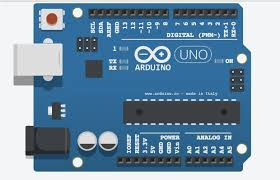
\includegraphics[width=0.4\textwidth]{figures/arduinounor3.jpg}}
\caption{Arduino UNO R3.}
\label{arduinounor3}
\end{figure}
Arduino UNO \ref{arduinounor3} adalah sebuah board mikrokontroler yang didasarkan pada ATmega328 (datasheet). Arduino UNO mempunyai 14 pin digital input/output (6 diantaranya dapat digunakan sebagai output PWM), 6 input analog, sebuah osilator Kristal 16 MHz, sebuah koneksi USB, sebuah power jack, sebuah ICSP header, dan sebuat tombol reset. Arduino UNO mempunyai komponen - komponen yang diperlukan untuk membuat sebuah mikrokontroler, mudah untuk menghubungkannya ke komputer melalui sebuah kabel USB atau menggunakan baterai atau menyuplainya dengan sebuah adaptor AC ke DC untuk memulainya.
Arduino Uno berbeda dari semua board Arduino sebelumnya, Arduino UNO tidak menggunakan chip driver FTDI USB-to-serial. Sebaliknya, fitur-fitur Atmega16U2 (Atmega8U2 sampai ke versi R2) diprogram sebagai sebuah pengubah USB ke serial. Versi ke-2 dari papan Arduino Uno memiliki satu buah resistor yang dapat menarik garis - garis 8U2 HWB ke ground serta mempermudahkannya untuk ditaruh ke mode DFU.
\subsection{Komputer + Software IDE Arduino}
\begin{figure}[ht]
\centerline{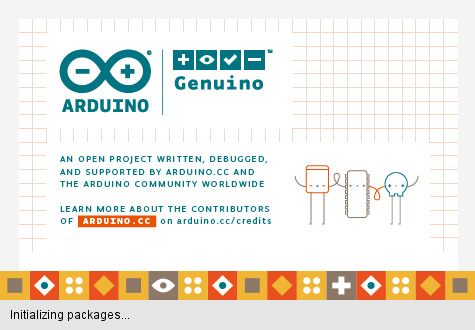
\includegraphics[width=0.4\textwidth]{figures/aride11.png}}
\caption{Arduino IDE.}
\label{aide}
\end{figure}
Menurut F. Djuandi dalam bukunya yang berjudul "Pengenalan Arduino" \cite{djuandi2011pengenalan} IDE merupakan singkatan dari Integrated Development Environment atau lingkungan terintegrasi yang digunakan untuk melakukan pengembangan. Melalui software inilah dilakukan pengembangan pemrograman Arduino yang nantinya melakukan fungsi - fungsi yang sudah ditanamkan melalui sintaks pemrograman. Tampilan IDE ini bisa dilihat pada gambar \ref{aide}. IDE ini disediakan gratis dan bisa didapatkan secara langsung pada halaman resmi arduino yang bersifat open source. IDE ini juga sudah mendukung berbagai sistem operasi populer saat ini seperti Windows, Mac, dan Linux. Arduino menggunakan bahasa pemrograman sendiri yang menyerupai bahasa C. Pada bahasa pemrograman Arduino (Sketch) telah dilakukan beberapa perubahan untuk memudahkan para pemula dalam melakukan pemrograman dari bahasa aslinya. Sebelum diperjualbelikan ke pasaran, IC microcontroller Arduino sebelumnya telah ditanamkan sebuah program yang bernama Bootlader yang memiliki fungsi sebagai penengah antara compiler Arduino dengan microcontroller.

\subsection{Modul Sensor Suara}
\begin{figure}[ht]
\centerline{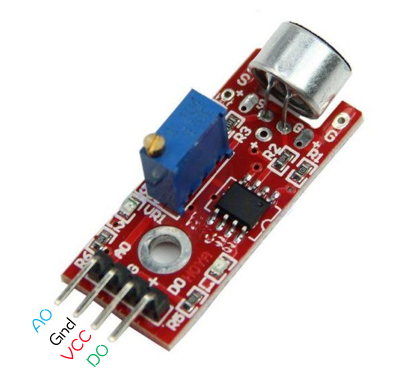
\includegraphics[width=0.4\textwidth]{figures/sssensorsuara.png}}
\caption{Modul Sensor Suara}
\label{sssensorsuara}
\end{figure}
Sensor suara merupakan sensor yang mensensing besaran suara untuk diubah menjadi besaran listrik. Sensor ini bekerja berdasarkan besar kecilnya kekuatan gelombang suara yang diterima. Dimana gelombang suara tersebut mengenai membran sensor, yang menyebabkan bergeraknya membran sensor yang memiliki kumparan kecil sehingga menghasilkan besaran listrik. Kecepatan bergeraknya kumparan kecil tersebut menentukan kuat lemahnya gelombang listrik yang akan dihasilkan. Salah satu contoh komponen yang termasuk dalam sensor ini adalah condeser microphone atau mic. Bentuk fisik dari condeser mic yaitu berbentuk bulat dan memiliki kaki dua seperti contoh pada gambar \ref{sssensorsuara}.
\subsection{Kabel Jumper}
\begin{figure}[ht]
\centerline{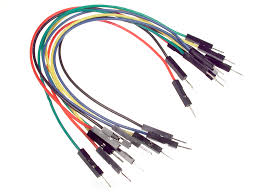
\includegraphics[width=0.4\textwidth]{figures/kabeljumper.jpg}}
\caption{Kabel Jumper.}
\label{kabeljumper}
\end{figure}
Kabel jumper seperti contoh pada gambar \ref{kabeljumper} adalah komponen yang wajib ada saat belajar rangkaian elektronika dan komponen penghubung rangkaian Arduino dengan breadboard. Hal-hal yang jadi masalah pada kabel jumper antara lain jumlahnya tidak punya banyak atau kabel jumper gampang rusak karena saat beli kualitas tidak diperhitungkan.
Kabel jumper memang banyak dijual dengan harga tertentu tergantung dengan kualitasnya, tetapi kabel jumper juga bisa dibuat sendiri dengan harga modal yang lebih murah dan menghasilkan jumlah kabel yang banyak meski tampilan berbeda dengan buatan pabrik tetapi secara fungsi, kabel jumper yang dibuat sendiri masih dapat berfungsi sebagaimana mestinya.

\subsection{Lampu LED}
\begin{figure}[ht]
\centerline{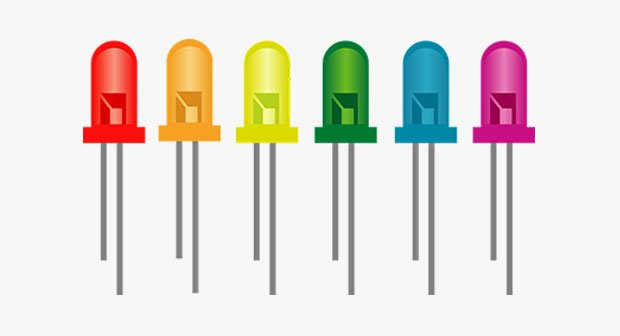
\includegraphics[width=0.4\textwidth]{figures/ledled.jpg}}
\caption{Lampu LED.}
\label{led}
\end{figure}
Light Emitting Diode atau sering disingkat dengan LED seperti contoh pada gambar \ref{led} adalah komponen elektronika yang dapat memancarkan  cahaya monokromatik ketika diberikan tegangan maju. LED termasuk ke dalam jenis dioda yang dibuat dari bahan - bahan semikonduktor. Warna-warna yang dipancarkan oleh cahaya LED tergantung dari jenis bahan - bahan semikonduktor yang dipergunakannya.


%%%%%%%%%%%%%%%%%%%%%%%%%%%%%%%%%%%%%%%%%%%%%%%%%%%%%%%%%%



Untuk membedakan yang mana terminal Katoda (-) dan terminal Anoda (+) pada LED, kita dapat mengetahuinya secara langsung. Ciri - ciri dari terminal Anoda (+) pada LED yaitu kakinya lebih panjang dan juga Lead Framenya lebih kecil. Sedangkan ciri-ciri Terminal Katoda ( - ) adalah kakinya lebih pendek dan juga Lead Framenya lebih besar serta terletak di sisi yang Flat.
\subsection{Kabel USB}
\begin{figure}[ht]
\centerline{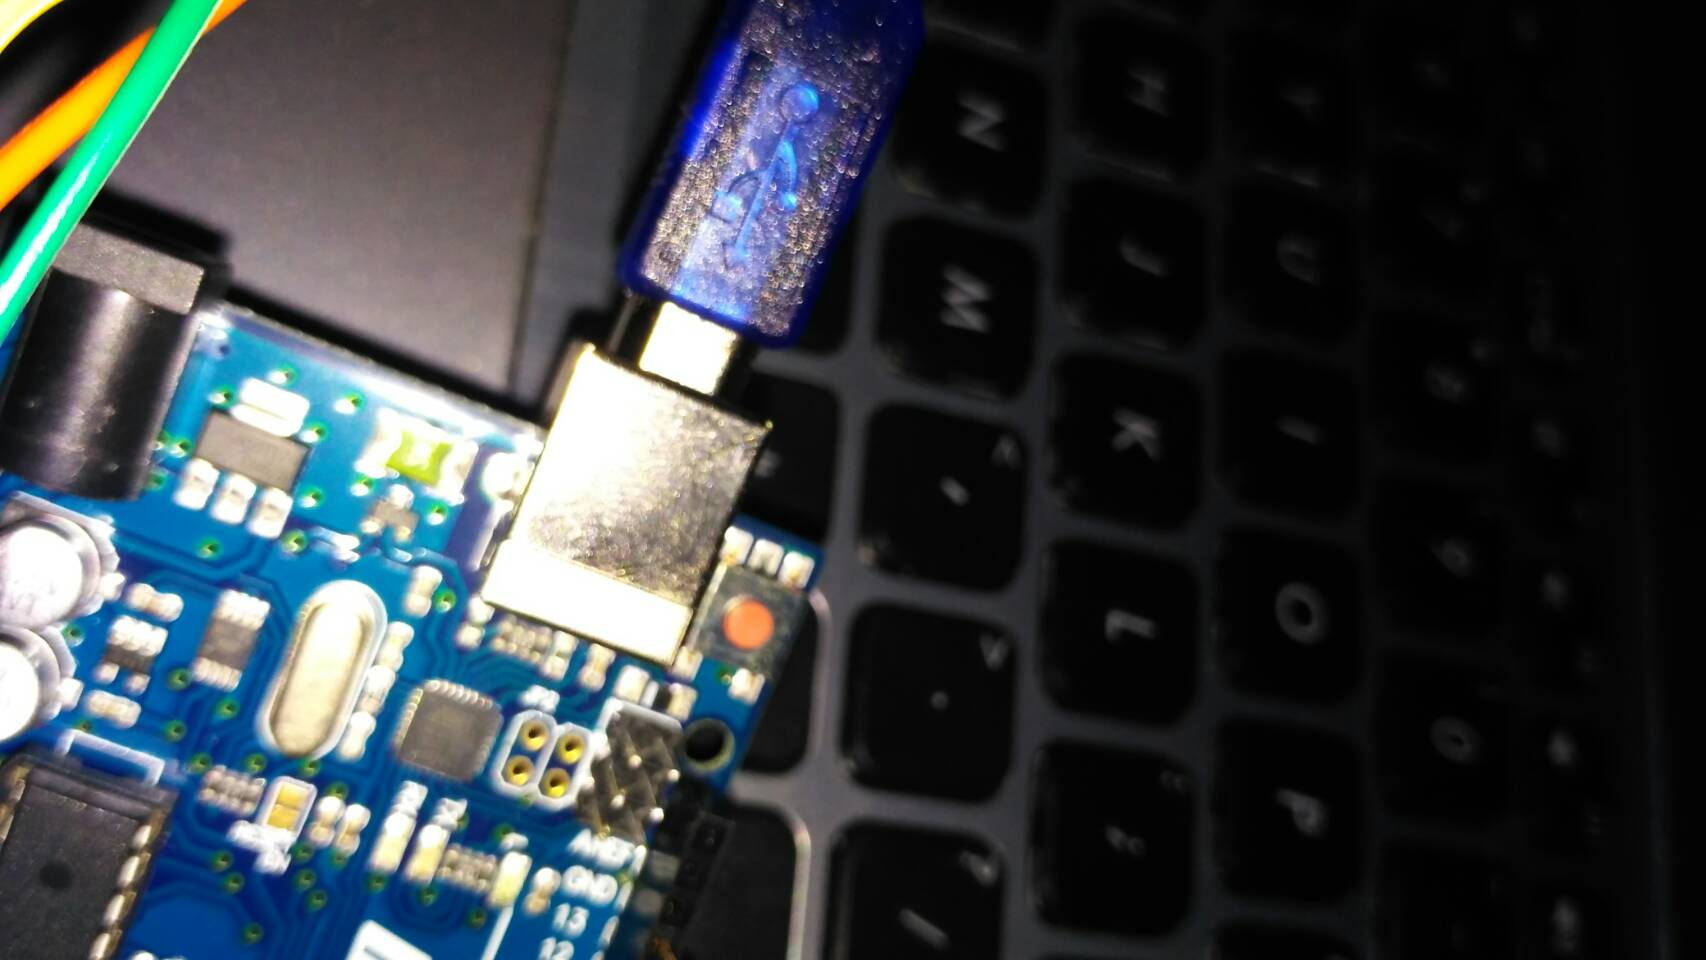
\includegraphics[width=0.4\textwidth]{figures/usb.jpg}}
\caption{Kabel USB.}
\label{usb}
\end{figure}
Kabel USB ( Universal Serial Bus ) seperti contoh pada gambar \ref{usb} merupakan pengkonversi pada arduino yang memiliki fungsi sebagai kabel untuk menghidupkan atau menjalankan arduino dan juga kabel ini memiliki fungsi sebagai media transfer untuk mengupload barisan kode - kode yang telah dibuat pada software arduino IDE.

\subsection{Bread Board}
\begin{figure}[ht]
\centerline{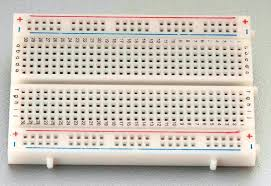
\includegraphics[width=0.4\textwidth]{figures/breadboard.jpg}}
\caption{Bread Board.}
\label{breadboard}
\end{figure}
Project Board atau yang sering disebut sebagai BreadBoard seperti contoh pada gambar \ref{breadboard} adalah dasar konstruksi sebuah sirkuit elektronik dan merupakan prototipe dari suatu rangkaian elektronik. Di zaman modernisasi istilah ini sering dipergunakan untuk merujuk pada jenis tertentu dari papan tempat merangkai komponen, dimana papan ini tidak memerlukan proses menyolder ( langsung tancap ).
Karena papan ini solderless alias tidak memerlukan solder sehingga dapat digunakan kembali, dan dengan demikian dapat digunakan untuk prototipe sementara serta membantu dalam bereksperimen desain sirkuit elektronika. Banyak dari sistem elektronik yang dibuatkan prototipe dengan mempergunakan project board atau breadboard, seperti digital kecil dan sirkuit analog serta CPU (Central Prossesing Unit).

\subsection{Resistor}
\begin{figure}[ht]
\centerline{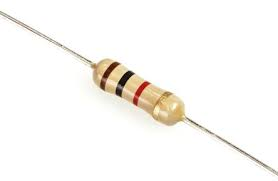
\includegraphics[width=0.4\textwidth]{figures/resistor.jpg}}
\caption{Resistor.}
\label{resistor}
\end{figure}
Resistor seperti contoh pada gambar \ref{resistor} merupakan komponen elektronik yang memiliki dua pin dan didesain untuk mengatur tegangan listrik dan arus listrik, dengan resistansi tertentu (tahanan) dapat memproduksi tegangan listrik di antara kedua pin, nilai tegangan terhadap resistansi berbanding lurus dengan arus yang mengalir, berdasarkan hukum Ohm.
Resistor digunakan sebagai bagian dari rangkaian elektronik dan sirkuit elektronik, dan merupakan salah satu komponen yang paling sering digunakan. Resistor terbuat dari berbagai macam komponen - komponen, seperti kawat resistansi atau kawat yang terbuat dari campuran resistivitas tinggi, contohnya nikel-kromium.



\subsection{Proses Instalasi IDE}

Berikut ini adalah proses instalasi IDE Arduino :

\begin{enumerate}
\item Pertama unduh terlebih dahulu installer IDE Arduino di https://www.arduino.cc/en/Main/Software. Pada halaman tersebut ada tiga macam installer yang dapat diunduh sesuai dengan Operating System yang kita pakai.
\break\\
\centerline{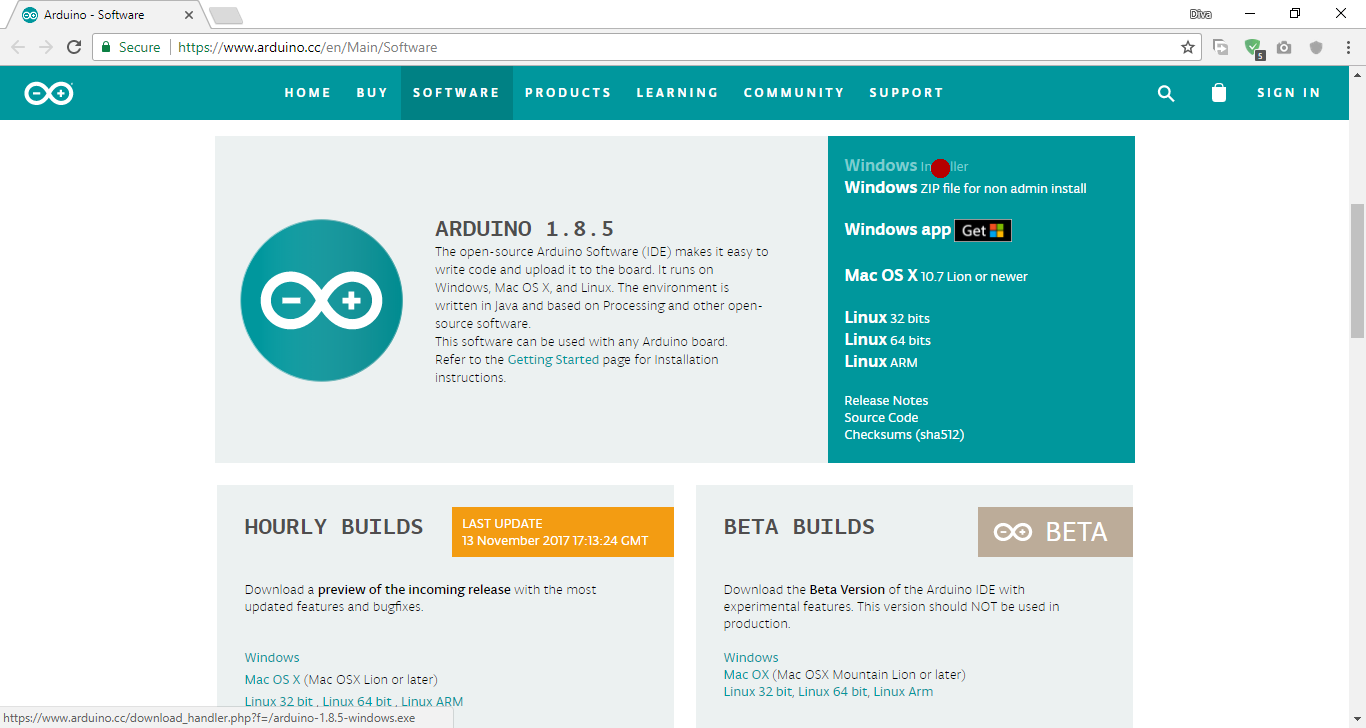
\includegraphics[width=0.9\textwidth]{figures/aride8.png}}
\item Kemudian pada halaman tersebut ada dua pilihan apakah kita ingin berkontribusi dengan memberikan uang sesuai dengan nominal yang tertera atau hanya mengunduh saja. Disini kita klik `Just Download' dan proses mengunduh dimulai.
\break\\
\centerline{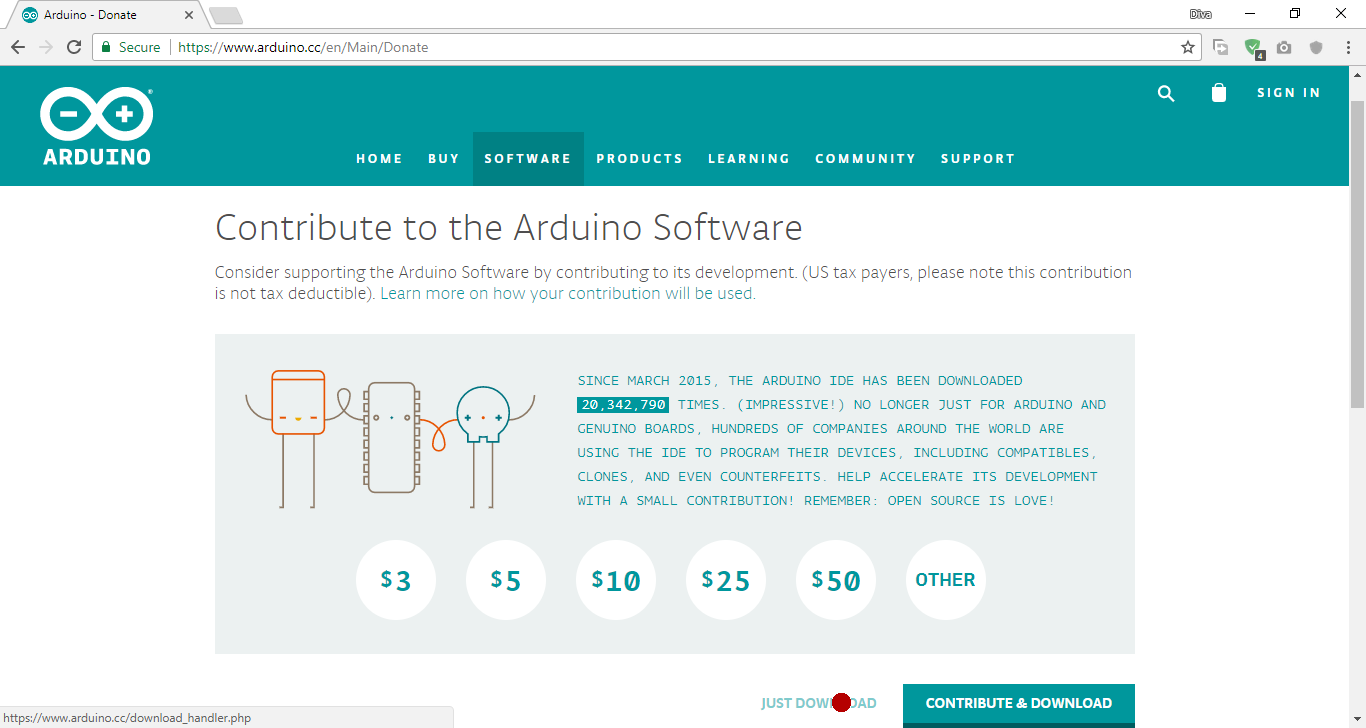
\includegraphics[width=0.9\textwidth]{figures/aride9.png}}
\item Setelah file installer telah selesai di unduh, lalu jalankan installer tersebut. Selanjutnya akan muncul jendela `Arduino Setup: License Agreement'. Lalu klik tombol `I Agree'.
\break\\
\centerline{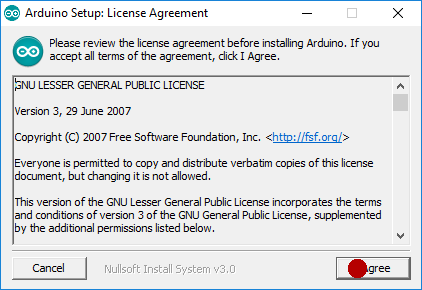
\includegraphics[width=0.9\textwidth]{figures/aride1.png}}
\item Selanjutnya akan muncul jendela `Arduino Setup: Installation Options'. Centang semua opsi yang ada, lalu klik `Next'.
\break\\
\centerline{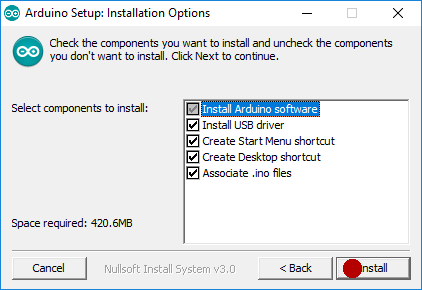
\includegraphics[width=0.9\textwidth]{figures/aride2.png}}
\item Setelah itu, akan muncul jendela `Arduino Setup: Installation Folder'. Kita diminta memilih folder instalasi Arduino.
\break\\
\centerline{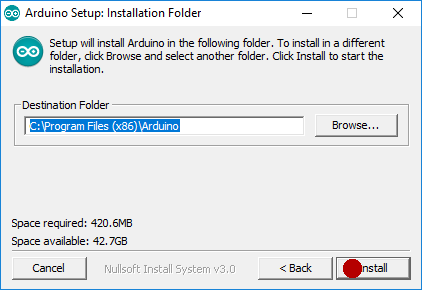
\includegraphics[width=0.9\textwidth]{figures/aride3.png}}
\item Selanjutnya proses instalasi akan dimulai.
\break\\
\centerline{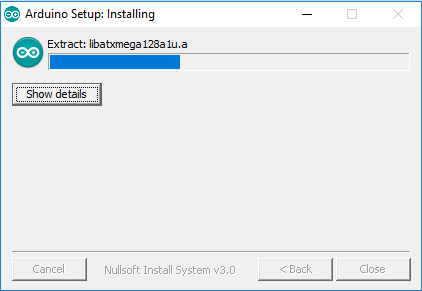
\includegraphics[width=0.9\textwidth]{figures/aride4.png}}
\item Pada saat melakukan proses instalasi, akan muncul jendela `Windows Security'. Jendela tersebut muncul apabila komputer kita belum terinstal driver - driver yang diperlukan. Klik tombol `Install'.
\break\\
\centerline{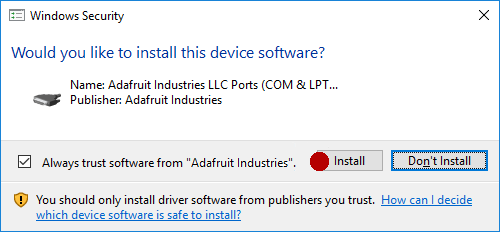
\includegraphics[width=0.9\textwidth]{figures/aride5.png}}
\break\\
\centerline{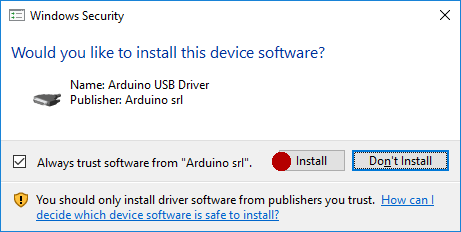
\includegraphics[width=0.9\textwidth]{figures/aride6.png}}
\break\\
\centerline{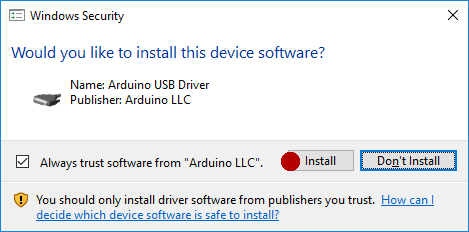
\includegraphics[width=0.9\textwidth]{figures/aride7.png}}
\item Selanjutnnya akan muncul jendela `Arduino Setup: Completed'. Jendela ini menandakan proses instalasi telah selesai. Klik tombol `Close'.
\break\\
\centerline{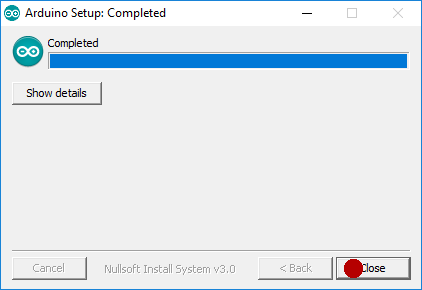
\includegraphics[width=0.9\textwidth]{figures/aride10.png}}
\item Setelah software IDE Arduino sudah terinstal. Coba cek di Start Menu Windows atau di desktop Anda, lalu jalankan aplikasi tersebut. Kemudian akan muncul splash screen seperti gambar di bawah ini.
\break\\
\centerline{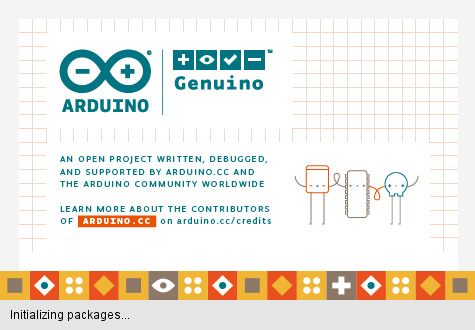
\includegraphics[width=0.9\textwidth]{figures/aride11.png}}
\item Selanjutnya akan muncul jendela IDE Arduino. Selamat Anda telah berhasil menginstal software IDE Arduino.
\break\\
\centerline{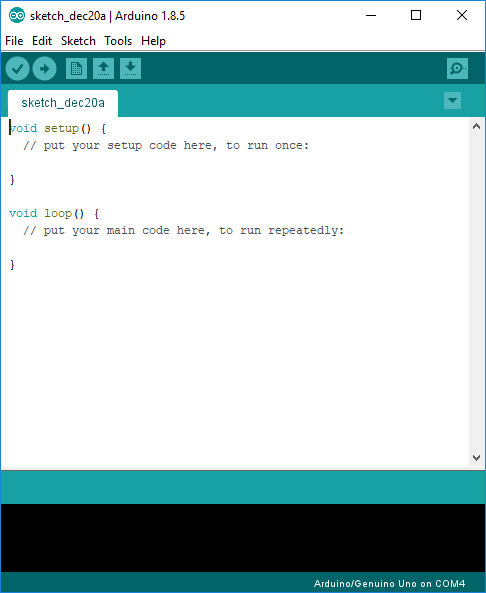
\includegraphics[width=0.9\textwidth]{figures/aride12.png}}
\end{enumerate}

\subsection{Proses Perakitan}

Berikut ini adalah langkah - langkah proses perakitan modul sensor suara dengan Arduino UNO :

\begin{enumerate}

\item  Pertama, pasang kabel jumper bagian female ke masing-masing pin modul sensor suara. Kabel jumper berwarna putih ke pin Analog Output (AO). Kabel jumper berwarna abu-abu ke pin Ground (G). Kabel jumper berwarna hitam ke pin Voltage Common Collector (VCC)/+.
\break\\
\centerline{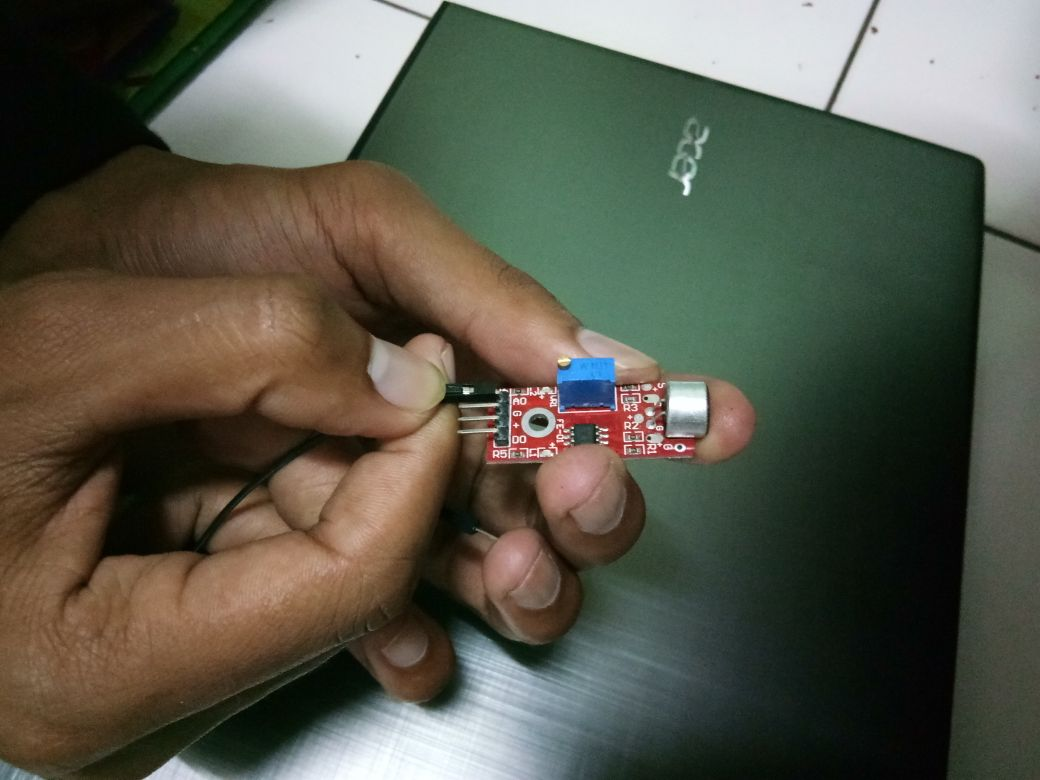
\includegraphics[width=0.9\textwidth]{figures/ss4.jpeg}}
\break\\
\centerline{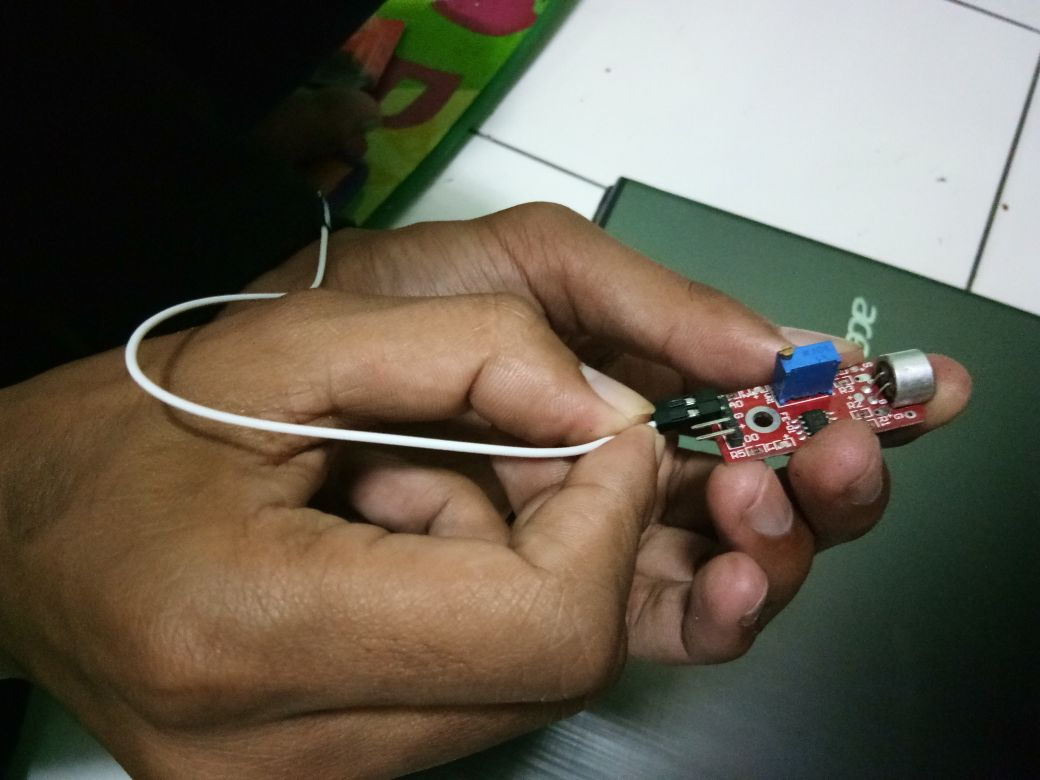
\includegraphics[width=0.9\textwidth]{figures/ss5.jpeg}}
\break\\
\centerline{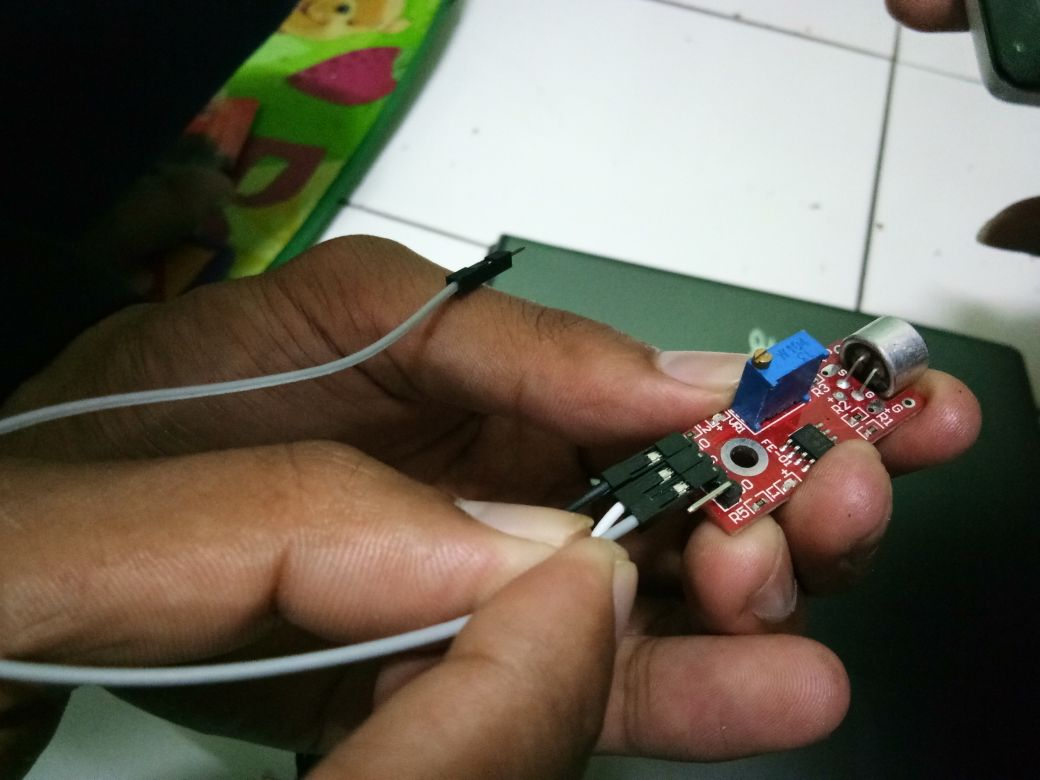
\includegraphics[width=0.9\textwidth]{figures/ss6.jpeg}}
\item Setelah semuanya terpasang, lalu sambungkan kabel jumper bagian male ke arduino. Kabel jumper berwarna putih ke slot A2. Kabel jumper berwarna abu-abu ke slot GND. Kabel jumper berwarna hitam ke slot 5V.
\break\\
\centerline{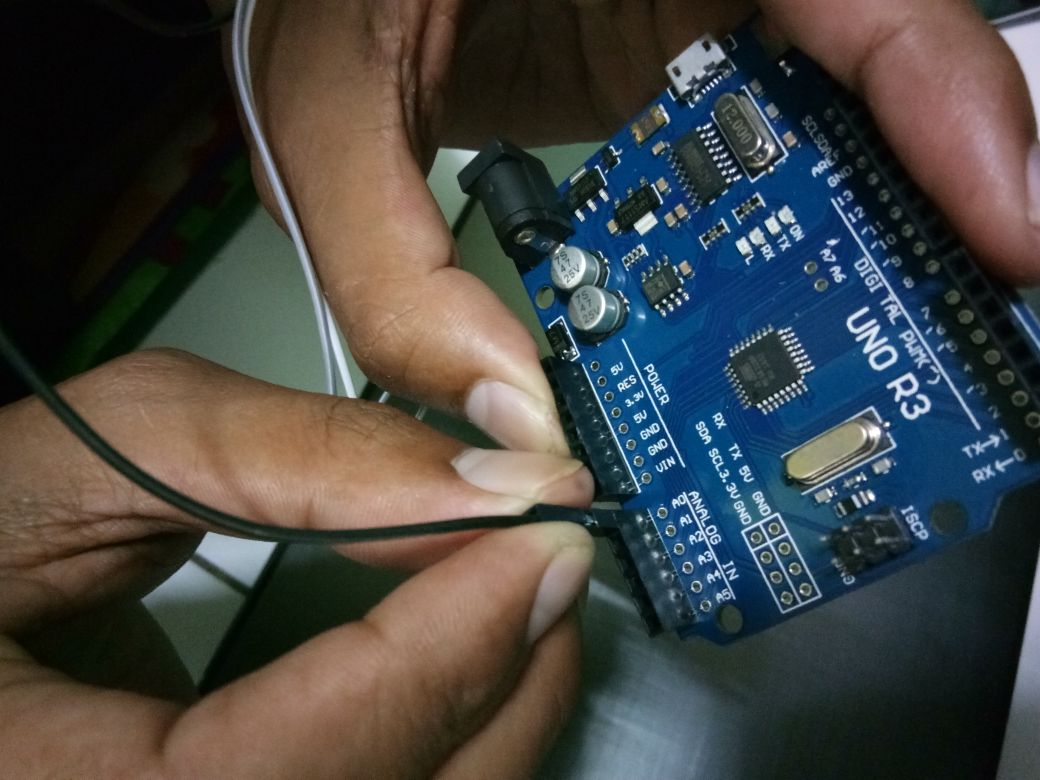
\includegraphics[width=0.9\textwidth]{figures/ss1.jpeg}}
\break\\
\centerline{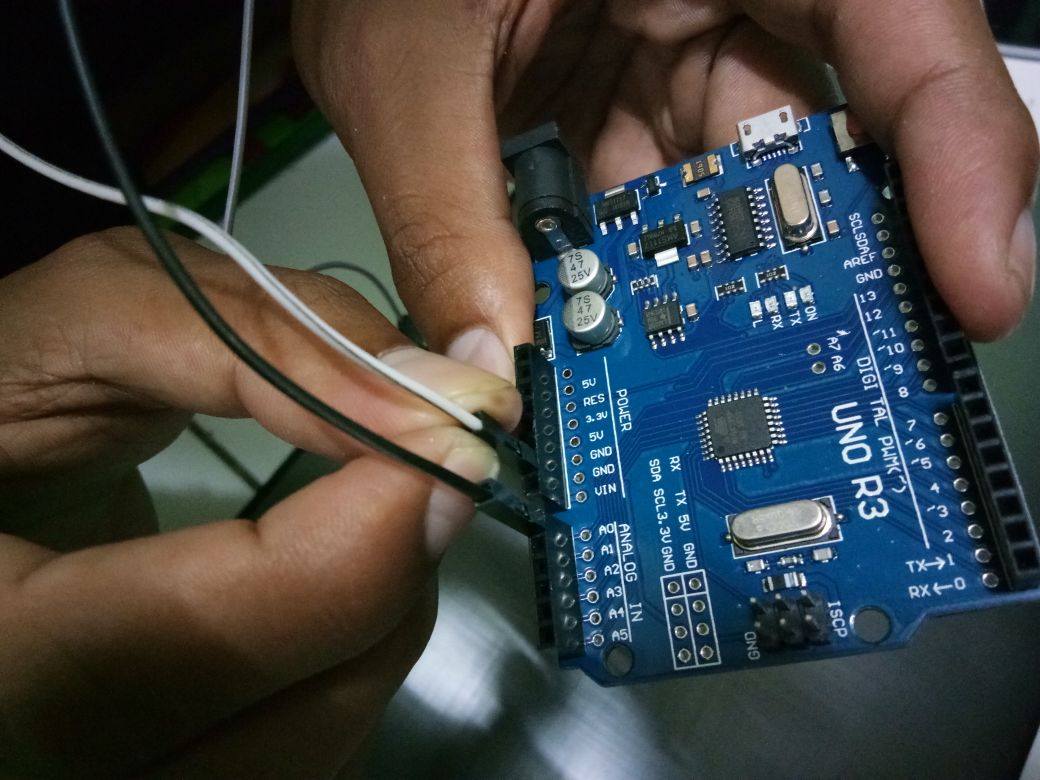
\includegraphics[width=0.9\textwidth]{figures/ss2.jpeg}}
\break\\
\centerline{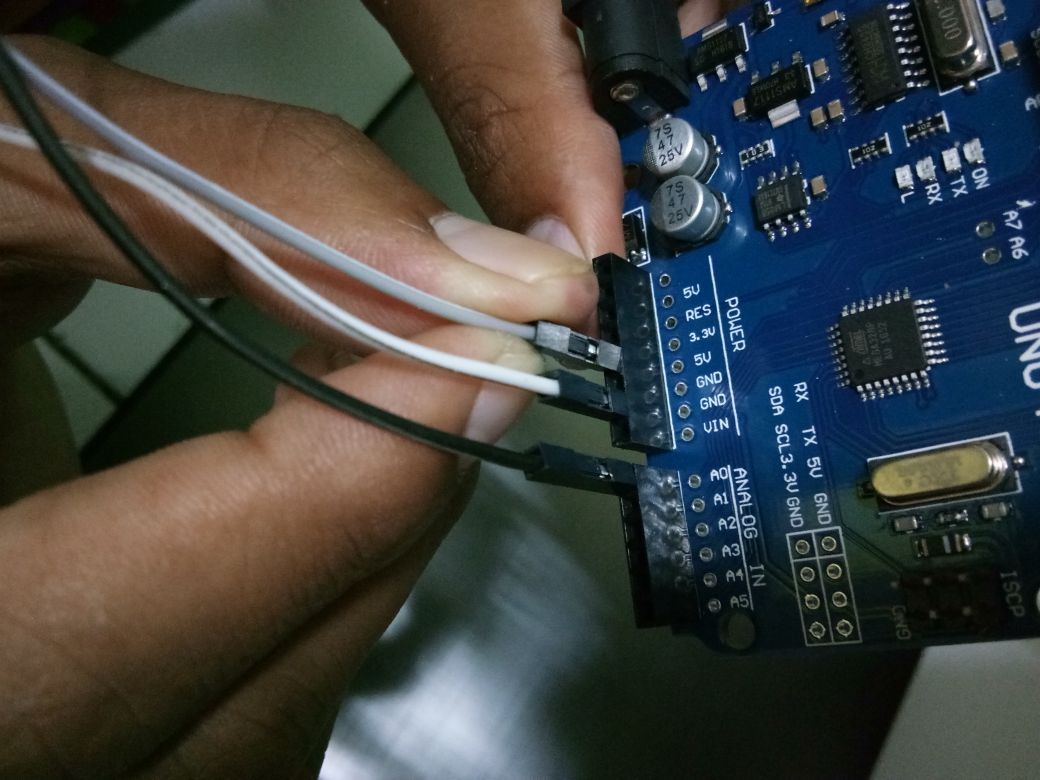
\includegraphics[width=0.9\textwidth]{figures/ss3.jpeg}}
\item Setelah semua terhubung, lalu sambungkan kabel USB ke arduino dan ke komputer.
\break\\
\centerline{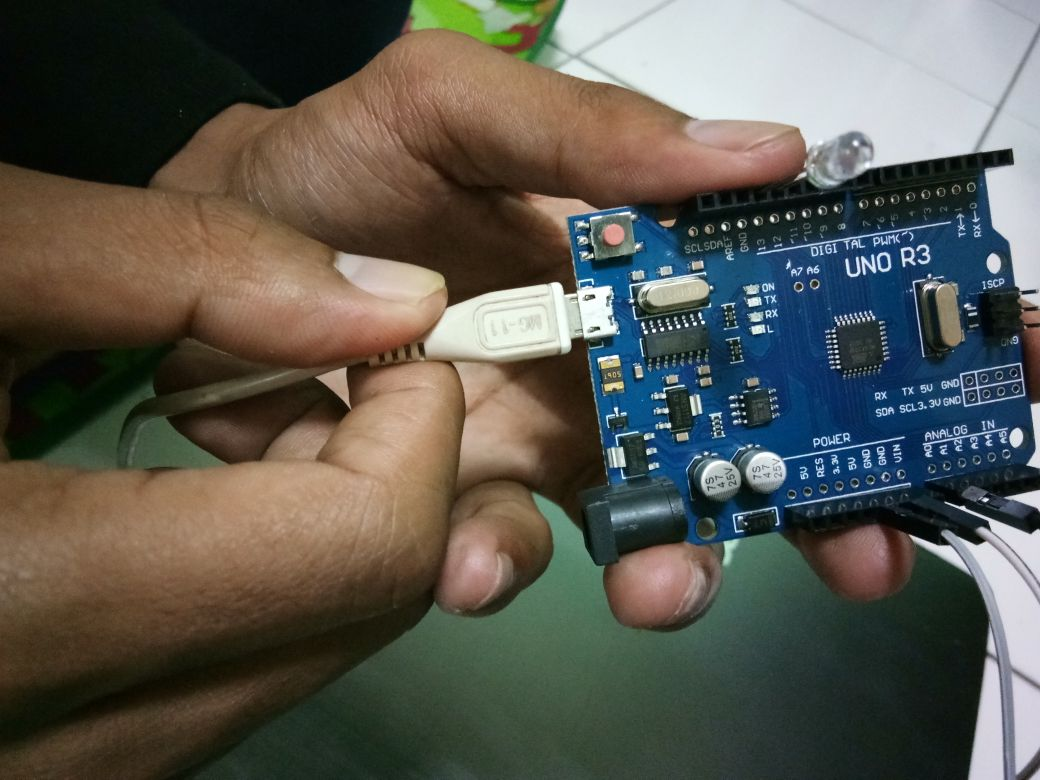
\includegraphics[width=0.9\textwidth]{figures/ss8.jpeg}}
\break\\
\centerline{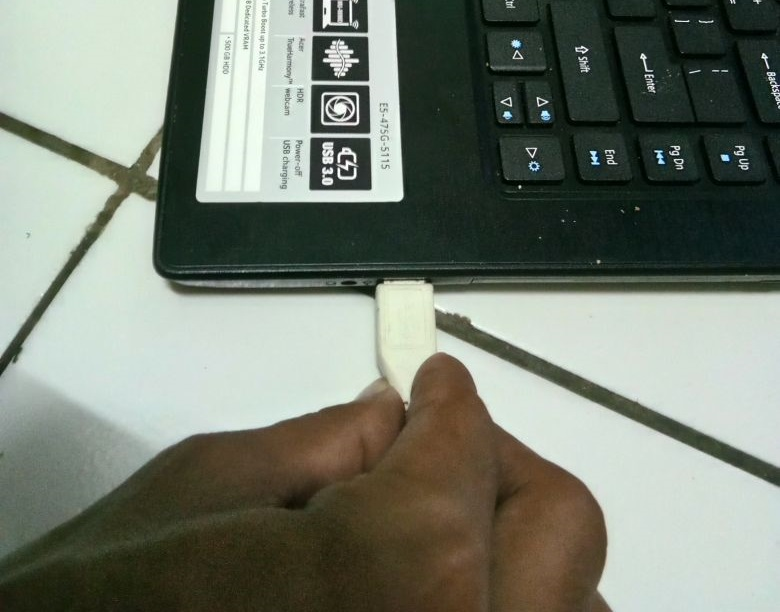
\includegraphics[width=0.9\textwidth]{figures/ss7.jpeg}}
\item Lalu pasang lampu LED ke arduino. Pin yang lebih panjang pasang ke slot 13, sedangkan pin yang pendek pasang ke slot GND.
\break\\
\centerline{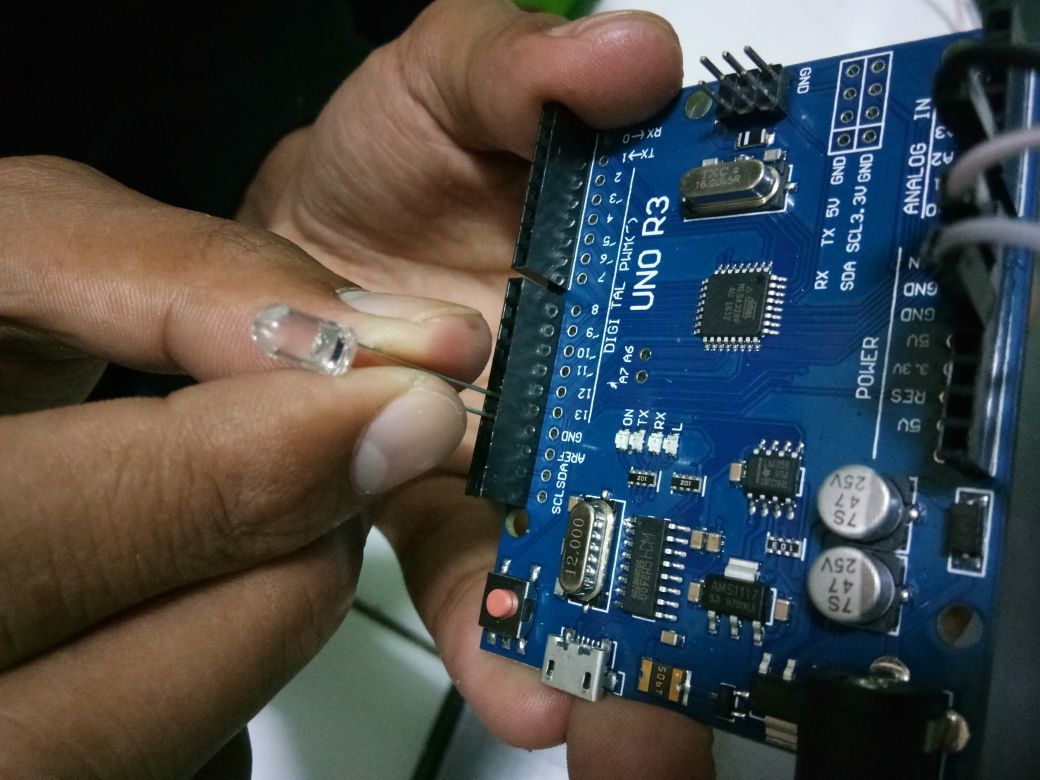
\includegraphics[width=0.9\textwidth]{figures/ss9.jpeg}}
\item  Kemudian buat program yang nantinya digunakan untuk mengetes sensor menggunakan IDE Arduino.
\break\\
\centerline{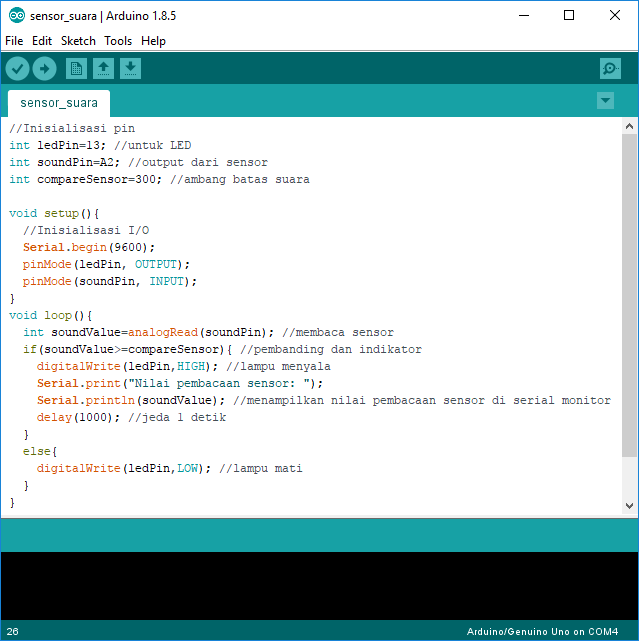
\includegraphics[width=0.9\textwidth]{figures/ss10.png}}
\break \textbf{Program Sensor Suara :}
\begin{verbatim}
//Inisialisasi pin
int ledPin=13; //untuk LED
int soundPin=A2; //output dari sensor
int compareSensor=27; //ambang batas suara

void setup(){
  //Inisialisasi I/O
  Serial.begin(9600);
  pinMode(ledPin, OUTPUT); //mengeluarkan keluaran
  pinMode(soundPin, INPUT); //menerima masukan
}
void loop(){
  int soundValue=analogRead(soundPin); //membaca sensor analog pin
    if(soundValue>compareSensor){ //pembanding dan indikator
    digitalWrite(ledPin,HIGH); //lampu menyala
    Serial.print("Nilai pembacaan sensor: ");
    Serial.println(soundValue); //menampilkan nilai pembacaan sensor di serial monitor
    delay(10); //jeda 1 detik
  }
  else{
    digitalWrite(ledPin,LOW); //lampu mati
  }
}
\end{verbatim}
\item Lalu setelah program selesai dibuat, unggah program tersebut ke arduino.
\break\\
\centerline{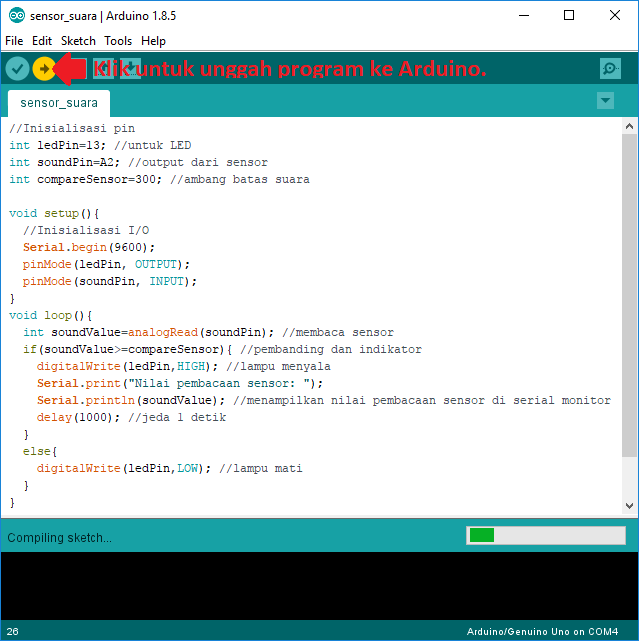
\includegraphics[width=0.9\textwidth]{figures/ss11.png}}
\item Terakhir cek apakah sensor berkerja dengan semestinya.
\break\\
\centerline{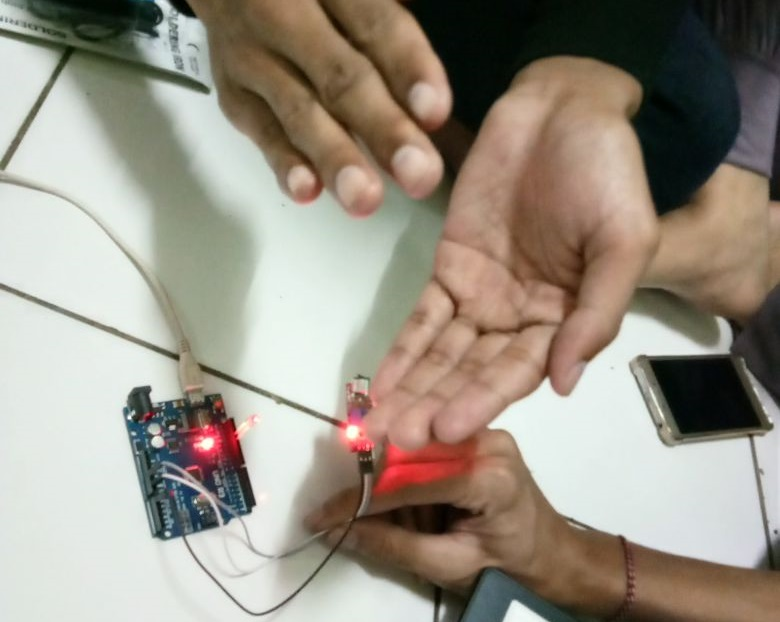
\includegraphics[width=0.9\textwidth]{figures/ss12.jpeg}}
\break\\
\centerline{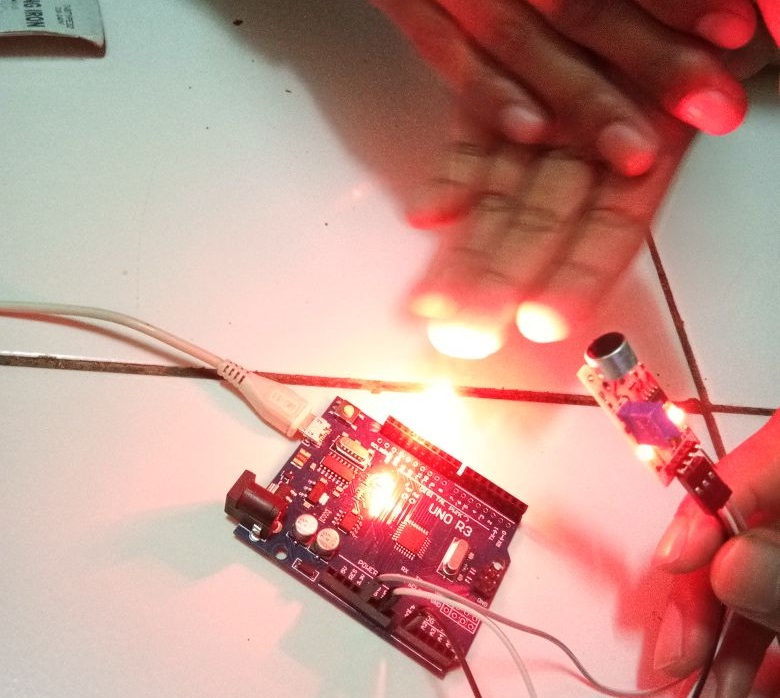
\includegraphics[width=0.9\textwidth]{figures/ss13.jpeg}}
\item Untuk mengecek nilai yang ditangkap oleh sensor, cek pada Serial Monitor.
\break\\
\centerline{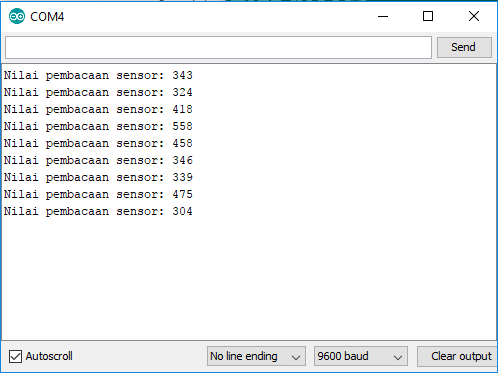
\includegraphics[width=0.9\textwidth]{figures/ss14.png}}

\end{enumerate}


%\end{document}
